\documentclass{article}
\usepackage[utf8]{inputenc}
\usepackage[dutch]{varioref}
\usepackage[autostyle]{csquotes} 
\usepackage[dutch]{babel}
\usepackage{pdfpages}
\usepackage{url}
\usepackage{natbib}
\usepackage{graphicx}

\title{Stageverslag}
\author{\mbox{Pieter-Jan} Robrecht}
\date{Maart 2016}

\begin{document}

%\maketitle
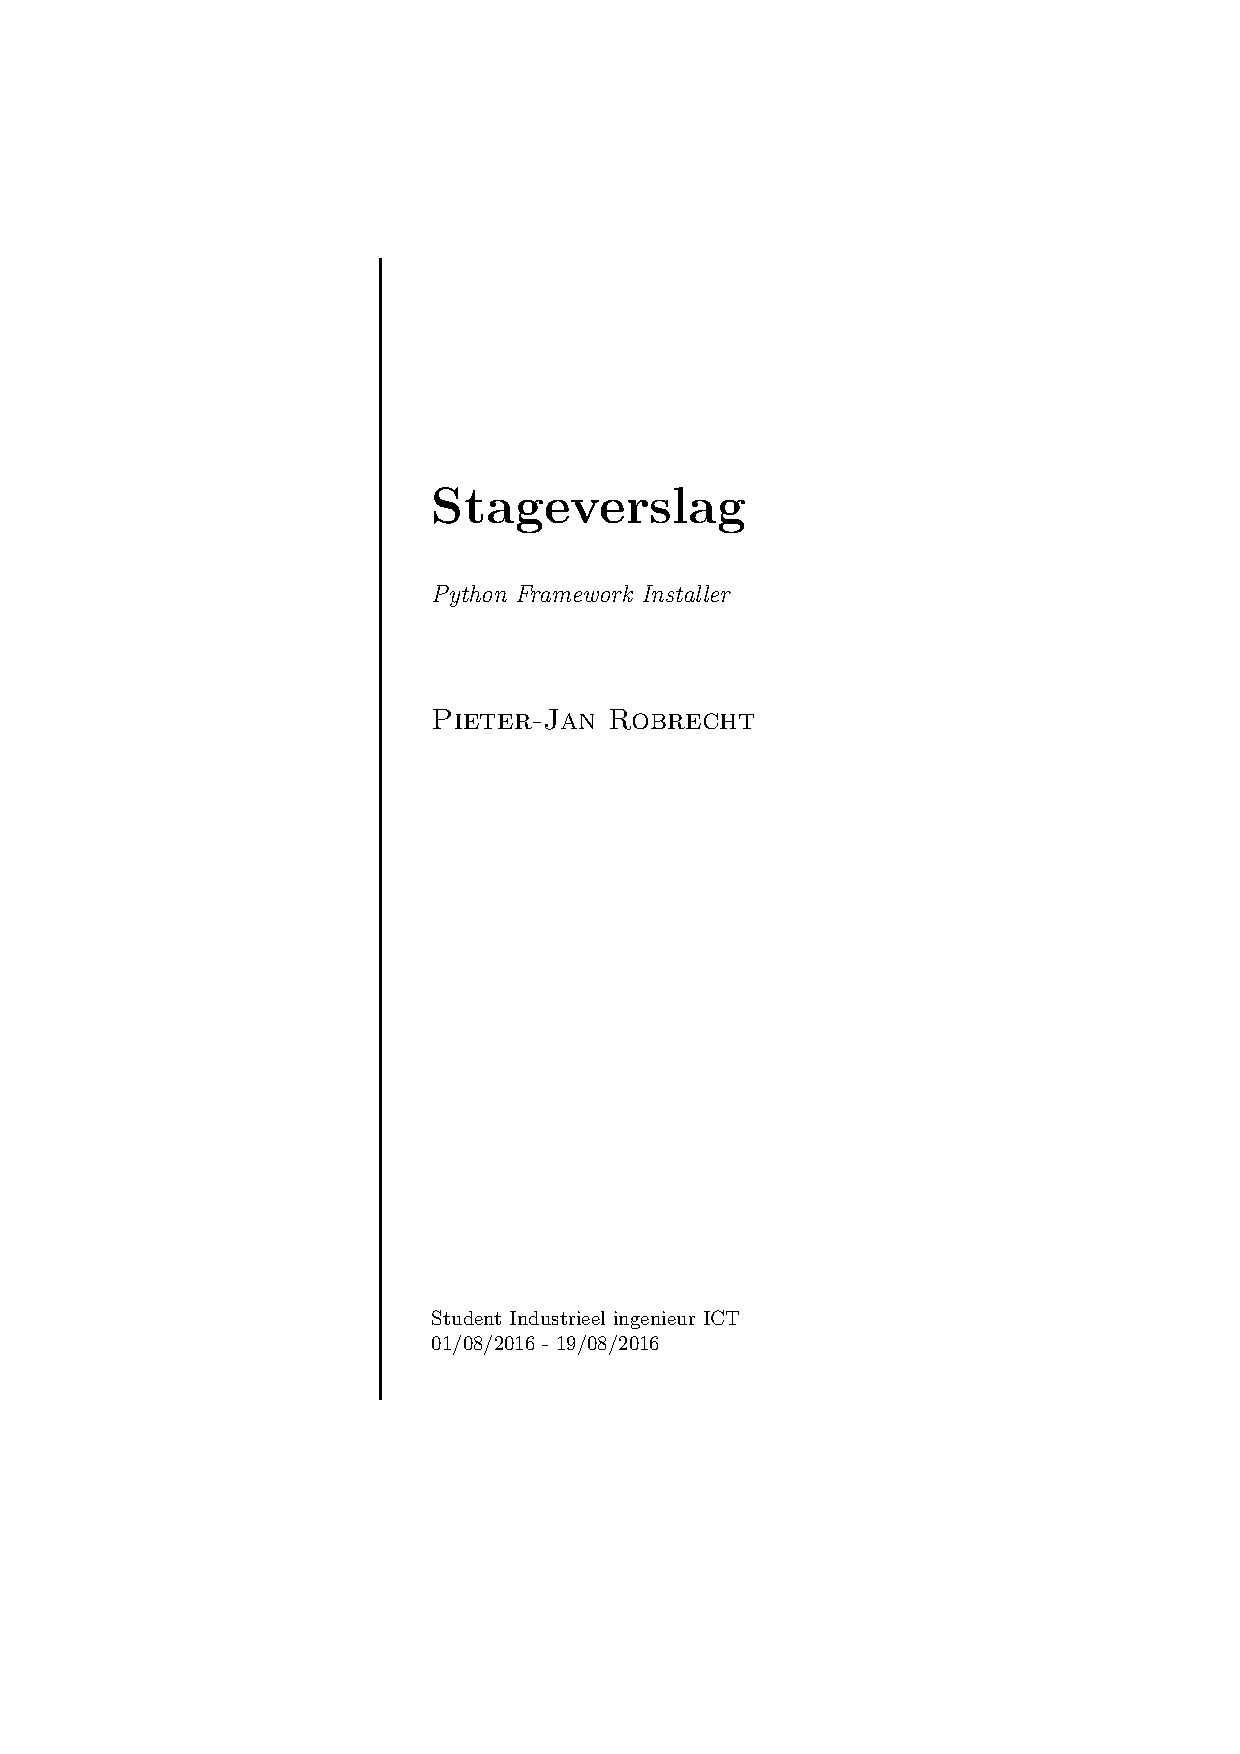
\includepdf{titel/titelstage.pdf}

%Volgende lijn is om de titelpagina geen paginanummer te geven
\clearpage
\setcounter{page}{1}

\tableofcontents
%\clearpage

\section{Inleiding}
In het kader van mijn masterproef was het mogelijk om bij Televic Rail een stage te lopen tijdens de zomer. 
Gedurende deze stage heb ik mijn masterproef voorbereid en onderzoek gedaan naar de verschillende mogelijkheden die er zijn voor het uitvoeren van mijn opdracht.
De opdracht die voltooid moet worden is de volgende:

\begin{displayquote}
Televic Rail heeft een Python test framework ontworpen. 
Dit framework werd oorspronkelijk gebruikt op een volledig uitgeruste testtoren, maar het framework werd aangepast zodanig dat het onafhankelijk van de testtoren gebruikt kan worden.
Aangezien het framework gebruik maakt van verschillende niet-standaard Python bibliotheken, is het installeren van het framework op een nieuw systeem een hele klus.
Het doel is dan ook het maken van een installer-updater waarmee dit proces kan worden vergemakkelijkt zodanig dat er zo min mogelijk interactie van de gebruiker moet zijn.
\end{displayquote}

Tijdens de duur van de stage werden de verschillende implementatie manieren onderzocht en werd er een algemene architectuur voor de installer-updater uitgedacht.
In wat volgt wordt er beschreven welke stappen er werden ondernomen om het probleem onder te verdelen in enkele logische onderdelen en hoe deze het probleem dan oplossen. 

\section{Analyse van het probleem}\label{section:analyse}
Tijdens het bespreken van het probleem werd het al snel duidelijk dat er verschillende scenario's zijn waarin het framework gebruikt wordt. 
Het framework wordt als een standalone programma gebruikt op een laptop of desktop maar het zal ook moeten draaien op verschillende testtorens. 
Voor de verschillende omgevingen zal iedere keer een andere configuratie nodig zijn maar beiden omgevingen gebruiken Windows als besturingssysteem.
Uiteraard moeten we ervan uitgaan dat deze situatie slechts tijdelijk is.
Er wordt best een applicatie geschreven die op verschillende types van systemen kan draaien.
Ook zorgen we er best voor dat het programma besturingssysteem-onafhankelijk is.

Tijdens het installeren van het framework moeten we rekening houden met het feit dat iedere computer een andere configuratie en andere drivers zal nodig hebben.
We zullen de gebruiker moeten vragen om de verschillende drivers te selecteren.
Mocht het mogelijk zijn dan zou er een mapping kunnen gebeuren tussen de verbonden devices en de nodige drivers zodanig dat deze automatisch worden aangevinkt in een selectielijst.
Het probleem van de drivers beperkt zich jammer genoeg niet enkel tot dit.
Als er nieuwe hardware ontwikkelt wordt, zullen er ook verschillende nieuwe drivers nodig zijn.
De lijst van beschikbare drivers zal dan tijdig moeten worden aangepast.

De installer is best ook een programma dat zo eenvoudig mogelijk uit te breiden is zodanig dat het in de toekomst nog kan worden aangepast. 
De interface naar de gebruiker toe is best ook zo eenvoudig mogelijk zodanig dat er geen problemen kunnen ontstaan tijdens de installatie van het framework.
Uiteraard gaan we er vanuit moeten gaan dat er af en toe een probleem zal ontstaan tijdens de installatie.
Updates zullen dus dan in een afgesloten omgeving moeten gebeuren en na het correct uitvoeren in het grote geheel geplaatst worden.

De updater bezit gelijkaardige problemen.
We zullen een manier moeten zoeken waarmee we gemakkelijk kunnen controleren naar de versienummers van de software.
De gebruiker zal ook de optie moeten krijgen om de update uit te voeren.
De gebruiker moet zelf beslissen wanneer de update uitgevoerd zal worden zodanig dat de update gebeurd als de gebruiker er klaar voor is.

\section{Oplossingen}
Aangezien we een algemeen beeld hebben van wat we juist allemaal moeten voorzien, kunnen we vervolgens aan de slag met het zoeken naar een goede oplossing voor alle problemen.
In wat hierna volgt gaan we alle mogelijkheden overlopen die gebruikt kunnen worden om de installer-updater te implementeren.
Alle verschillende opties gaan worden overlopen en de verschillende voor- en nadelen zullen besproken worden\footnote{Uiteraard is het mogelijk dat tijdens de duur van de masterproef nog mogelijk oplossingen worden gevonden.
In sectie~\vref{section:mogelijkheden} worden enkel de oplossingen besproken die tijdens de stage zijn gevonden.}.
Van hieruit gaan we ook een opsplitsing maken tussen de installer en de updater.
We gaan bij het zoeken naar een oplossing wel een opdeling maken tussen de oplossingen voor de installer en voor de updater.
Voor beiden zijn er oplossingen aanwezig en er zal gekeken moeten worden welke combinaties mogelijk zijn.

\subsection{Mogelijkheden}\label{section:mogelijkheden}
Laten we eerst kijken naar de besturingssysteem-onafhankelijkheid van het framework.
De besturingssysteem-onafhankelijkheid van Pyhton hangt af van de code en van de bibliotheken die gebruikt worden.
Zolang deze bibliotheken onafhankelijk zijn van het besturingssysteem is er geen enkel probleem.
Java biedt ook een oplossing aan voor dit probleem aangezien Java ook volledig besturingssysteem-onafhankelijk is.
Jammer genoeg zijn er amper tot geen programma's die een installer/updater kunnen genereren in Java.
Alle code voor zo'n programma zal zelf geschreven moeten worden.

\subsubsection{Qt Installer Framework \citep{qtDoc}}
Het Qt framework zou in staat zijn om eenmalig installers te maken die vervolgens op de ondersteunde platforms zou kunnen draaien.
De ondersteunde platforms zijn: Linux, Microsoft Windows en OS X \citep{qtOverview}.
De software zou de gebruiker door het installatie, update en verwijderproces leiden.
De programmeur moet enkel de nodige informatie over de te installeren software.
Er kunnen scripts geschreven worden voor de installer zodanig dat er verschillende opties toegevoegd kunnen worden.
bij iedere component kan een script toegevoegd worden zodanig dat de installatie kan worden gepersonaliseerd \citep{qtDocScript}.

Het Framework biedt twee types installers aan: een online en een offline installer.
Beide installers zullen een maintenance tool installer die gebruikt kan worden om componenten te updaten, toevoegen en verwijderen.
Het verschil tussen de twee installers is het volgende: de offline installer zal alle nodige componenten bevatten in de installer.
De online installer moet tijdens de installatie een verbinding maken met een online repository waar de nodige componenten worden gedownload. 
Bij de offline installer zullen alle componenten ge\"installeerd worden terwijl bij de online installer de keuze is om verschillende componenten niet te installeren \citep{qtOverview}.

Er zal wel moeten gekeken worden of dit een goede oplossing is voor ons probleem.
Tijdens de installatie van het framework en drivers wordt er gebruik gemaakt van verschillende windows executables. 
De installer zal deze moeten uitvoeren en tot een goed einde brengen.
De grote vraag is dan: is het mogelijk om een installer te maken met deze executables in die ook draait op Linux?
De installer zal ook de verschillende zip files moeten kunnen uitpakken en de setup uitvoeren.

\subsubsection{WiX \citep{wixMain}}
Windows Installer XML Toolset is een toolset waarmee Windows Installer packages gemaakt kunnen worden vanuit XML code.
WiX valt onder de Microsoft Reciprocal License \citep{wixLicense}.
Met de toolset is het mogelijk om een installer met als extensie .msi te maken.
Hiernaast is het ook mogelijk om patches te schrijven en code van andere te includeren dankzij merge modules\citep{wixMergers}.
Uitgaande van de eerste indruk, is het goed mogelijk dat deze genoeg opties aanbiedt om een degelijke installer te maken.
Hiernaast moet het ook mogelijk zijn om dankzij het patch systeem updates uit te voeren.
Er zal wel moeten gecontroleerd worden of dit systeem volautomatisch is.
Als dit niet zo is, dan zal er gekeken moeten worden hoe een updater kan worden ge\"implementeerd zodanig dat er geen nieuwe code moet geschreven worden bij iedere update.

\subsubsection{NSIS \citep{nsisMain}}
Nullsoft Scriptable Install System is een opensource systeem waarmee Windows installers kunnen gemaakt worden.
De overhead die NSIS zou cre\"eeren zou klein zijn maar dit zal uiteraard moeten gecontroleerd worden. 
NSIS is script-based en bied verschillende features aan die handig kunnen zijn voor deze toepassing \citep{nsisFeatures}.
Net zoals WiX zal de het script van NSIS een installer generen en vervolgens kan deze dan gebruikt worden voor de initi\"ele installatie.

\subsubsection{Chocolatey \citep{chocoMain}}
Chocolatey is een Powershell execution engine dat gebruikt maakt van de NuGet packaging infrastructuur.
Het systeem is te vergelijken met de package manager apt-get van linux.
Chocolatey zal alle executables, zips, ... die nodig zijn voor een stuk software encapsuleren zodanig dat alles in \'e\'en package zit.
Het packaging framework verstaat ook alle versioning en dependency requirements, iets dat zeker nodig is bij dit probleem \citep{chocoDoc}.
Chocolatey biedt verschillende mogelijkheden zodanig dat installatie, upgrades en verwijdering van het programma in de handen van de programmeur liggen.
Een mogelijk nadeel van deze methode is het gebruik van Powershell. 
De gebruikers zullen overweg moeten kunnen met Powershell en dit kan voor problemen zorgen. 

\paragraph{}
Nu dat alle verschillende opties globaal zijn besproken, is het belangrijk dat deze ook worden uitgetest zodanig dat er een duidelijk beeld kan gevormd worden over de mogelijkheden die ze effectief aanbieden.
In de volgende sectie zal een korte opsomming van de eisen een duidelijk beeld vormen over de verwachtingen van alle oplossingen.
Vervolgens zal er, aan de hand van een kleine test, gekeken worden of de oplossingen voldoen aan de eisen en naar welke de voorkeur uitgaat.
Nadat alle verschillende mogelijkheden zijn overlopen zijn, kan er een algemene architectuur van het programma opgesteld worden.

%\subsection{Testen}
%Zoals we in sectie~\vref{section:analyse} hebben besproken, zitten we met verschillende eisen waaraan de uiteindelijke oplossing moet voldoen.
%We gaan nu kort de verschillende eisen overlopen om vervolgens te bespreken hoe we deze eisen gaan testen bij de verschillende oplossingen die we in sectie~\vref{section:mogelijkheden} hebben aangehaald.
%Zoals reeds vermeld, zien we de installer en updater als twee verschillende entiteiten.
%Onze installer zal aan de volgende eisen moeten voldoen.
%De installer moet:
%\begin{itemize}
%\item registreren welk drivers ge\"instaleerd moeten worden.
%\item de optie geven om extra drivers te installeren.
%\item de meest recente versie van het framework downloaden.
%\item de nodige programma's in de correcte volgorde installeren.
%\item de interface moet zo eenvoudig mogelijk zijn.
%\item \'e\'en executable produceren, namelijk de updater.
%\item een eenmalige internetverbinding opzetten voor het downloaden van de nodige bestanden.
%\end{itemize}
%Dit moet allemaal gelogd worden zodanig dat bij fouten eenvoudig kan nagegaan worden waar de fout zit.
%
%Naast de installer hebben we ook de updater. Deze zal hoogst waarschijnlijk ge\"installeerd worden door de installer.
%De gebruiker zal voornamelijk met dit onderdeel in aanmerking komen.
%De updater moet zeker voldoen aan de volgende eisen.
%De updater moet:
%\begin{itemize}
%\item bij opstarten controleren of de versie van de drivers en het framework de meest recente is.
%\item een optie voorzien om handmatig nieuwe drivers te selecteren.
%\item een optie voorzien om het framework op te starten.
%\item bij iedere opstart zal een internetverbinding nodig zijn zodanig dat de nodige versiecontroles kunnen uitgevoerd worden.
%\end{itemize}
%De updater zal, net zoals de installer, een executable zijn.
%
%We zullen beginnen met het onderzoeken van de installer mogelijkheden.
%Tijdens het testen gaan we kijken of de installer een internetverbinding kan maken, een .exe file kan installeren en verschillende zips kan uitpakken en installeren.
%\subsection{Architectuur}

%Alfabetische volgorde
\bibliographystyle{plain}
%Orde van bib file
%\bibliographystyle{unsrt}
\bibliography{bib/stagebib}

\end{document}